\documentclass{standalone}
\usepackage{tikz}
\usepackage{xcolor}
\usepackage{./preamble}
\usepackage[sfdefault]{FiraSans}

\usetikzlibrary{decorations.pathreplacing}
\definecolor{mygreen}{RGB}{44,160,44}
\definecolor{myorange}{RGB}{255,127,14}
\definecolor{myred}{RGB}{214,39,40}
\definecolor{myorred}{RGB}{234,83,27}

\definecolor{mygrey}{HTML}{7F7F7F} %https://stackoverflow.com/questions/64369710/what-are-the-hex-codes-of-matplotlib-tab10-palette
\definecolor{myblue}{HTML}{1f77b4} %https://stackoverflow.com/questions/64369710/what-are-the-hex-codes-of-matplotlib-tab10-palette

\tikzstyle{mynode}=[align=center, rounded corners, draw=mygreen!30, minimum height = 1.cm, minimum width = 2cm,fill=mygreen!10]
\tikzstyle{mynodeorange}=[align=center, rounded corners, draw=myorange!30, minimum height = 1.cm, minimum width = 2cm,fill=myorange!10]
\tikzstyle{mynodered}=[align=center, rounded corners, draw=myred!30, minimum height = 1.cm, minimum width = 2cm,fill=myred!10]
\tikzstyle{mynodeblue}=[align=center, rounded corners, draw=myblue!30, minimum height = 1.cm, minimum width = 2cm,fill=myblue!10]

\tikzstyle{procs_ecolo}=[mynode, rectangle, fill=mygreen!30]


\begin{document}
\begin{tikzpicture}[
    module/.style={draw, very thick, rounded corners, minimum width=15ex},
    embmodule/.style={module, fill=red!20},
    mhamodule/.style={module, fill=orange!20},
    lnmodule/.style={module, fill=yellow!20},
    ffnmodule/.style={module, fill=cyan!20},
    % arrow/.style={-stealth', thick, rounded corners},
    arrow/.style={-stealth', very thick, rounded corners},
    node distance=0.5cm,
    every node/.style={font=\Large}
  ]

    \node[] (SAR) at (-14, 9) {\huge{Expected species-area relationship}};
    \node[] (SAR) at (-15, -3.5) {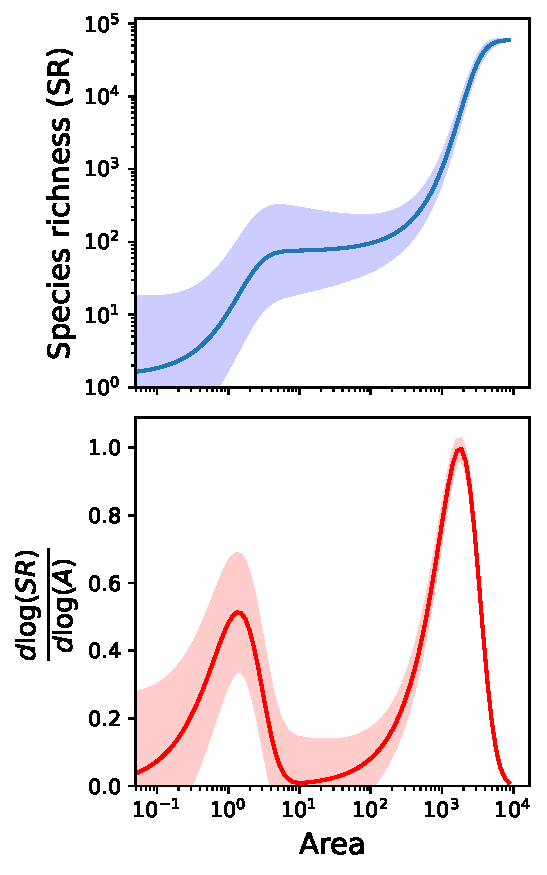
\includegraphics[width=14cm]{../conceptual_SAR.pdf}};
  
    \node[] (SAR) at (6, 9) {\huge{Vegetation plot augmentation scheme}};
    \node[mynode, minimum height=7cm, minimum width=7cm] (box2) at (-1.5, 3.8) {};
    \node[] (box_text) at (-2.8, 7) {Raw plot data};
    \node (lc) at(-1, 3.5) {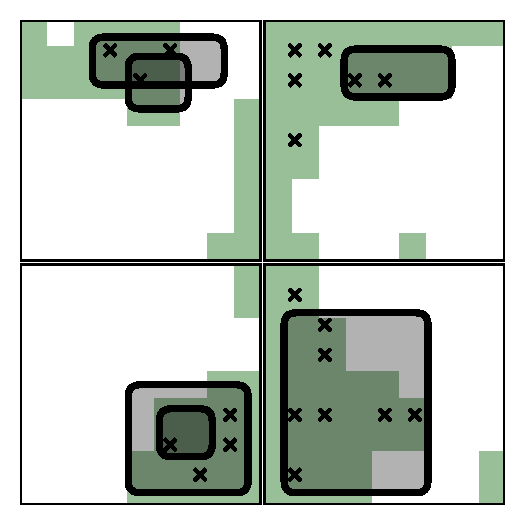
\includegraphics[width=6.2cm]{../panels/landcover_real.png}};

    \node[mynodeorange, minimum height=13.5cm, minimum width=7.6cm] (box) at (-1.8, -6.8) {};
    \node[] (box_text) at (-2., -0.5) {Raw environmental data};
    \node (cl1) at (-1.8, -4.0) {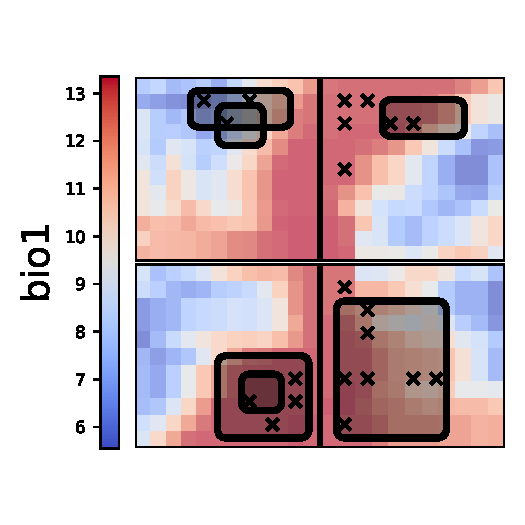
\includegraphics[width=7.8cm]{../panels/chelsa_real_bio1.png}};
    \node (cl2) at (-1, -7.25) {$\vdots$};
    \node (cl3) at (-1.8, -10.5) {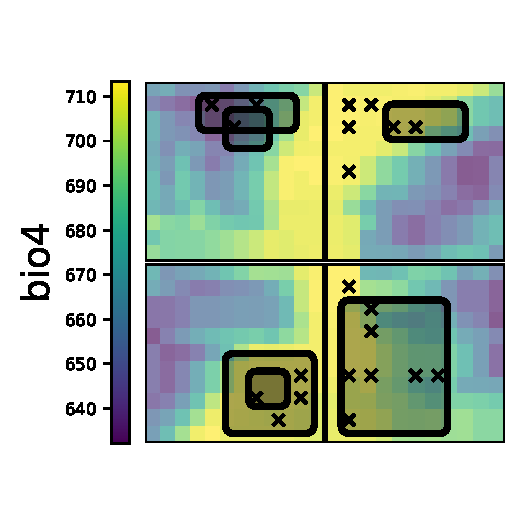
\includegraphics[width=7.8cm]{../panels/chelsa_real_bio4.png}};

    \node[align=center] (avp) at (7, 6.0) {Augmented vegetation plot $j$\\(megaplot)};
    \node (vp) [below=0.1cm of avp] {Vegetation plot $i$};
    \node (hm) [below=0.1cm of vp] {Habitat mask};
    \node (sb) [below=0.1cm of hm] {Spatial block};

    \draw ([xshift=-1cm,yshift=2.3cm]lc.east) to (avp.west);
    \draw ([xshift=-1.75cm,yshift=2.1cm]lc.east) to (vp.west);
    \draw ([xshift=-2.6cm,yshift=1.2cm]lc.east) to (hm.west);
    \draw ([xshift=-0.4cm,yshift=0.46cm]lc.east) to (sb.west);



  %   \draw [decorate,very thick,decoration={brace,amplitude=5pt,mirror,raise=4ex}]
  % ([xshift=-2.2cm, yshift=-3.2cm]lc.north) -- ([xshift=-2.2cm,yshift=0.4cm]lc.south) node[midway,xshift=-4em,rotate=90]{\normalsize 100km};

    % \node (sar) at (13,-1) {\includegraphics[width=14cm]{sar.png}};
    
    \node[mynode] (SR) [right=1cm of lc,yshift=-2cm] {$\text{SR}_j = |\cup_i \text{Species}_i|$};
    \node[mynode] (Area) [below =0.2cm of SR] {$\text{A}_j = \sum_i \text{Area}_i$};

    \node[mynodeblue] (mean1) [right=2cm of cl1,yshift=-1cm] {$\text{Mean}(\text{Bio1}_j)$};
    \node[mynodered] (std1) [below=0.2cm of mean1] {$\text{Std}(\text{Bio1}_j)$};
    \node[] (dots) [right=6.5cm of cl2] {$\vdots$};
    \node[mynodeblue] (mean2) [right=2cm of cl3,yshift=2cm] {$\text{Mean}(\text{Bio4}_j)$};
    \node[mynodered] (std2) [below=0.2cm of mean2] {$\text{Std}(\text{Bio4}_j)$};

    \node[mynode, draw=mygrey!30, fill=mygrey!10, align=center] (model) [right=6cm of dots, yshift=3cm] {\huge{Neural SAR} \\ \huge{model}\\[1em] \huge{$\mathcal{M}(X_j) = \hat{SR}_j$}};
    \node[mynodeorange, align=center] (physics) [below=2cm of model] {Physics-informed\\constraint\\[1em] \Huge{$\frac{\partial \mathcal{M}}{\partial A} > 0$}};



    \draw[arrow] ([xshift=-1.3cm,yshift=-1.5cm]lc.east) to[out=0, in=180] (SR.west);
    \draw[arrow] ([xshift=-1.3cm,yshift=-1.5cm]lc.east) to[out=0, in=180] (Area.west);
    
    \draw[arrow] ([xshift=-1.3cm,yshift=-1.4cm]cl1.east) to[out=0, in=180] (mean1.west);
    \draw[arrow] ([xshift=-1.3cm,yshift=-1.4cm]cl1.east) to[out=0, in=180] (std1.west);

    \draw[arrow] ([xshift=-1.3cm,yshift=-1.4cm]cl3.east) to[out=0, in=180] (mean2.west);
    \draw[arrow] ([xshift=-1.3cm,yshift=-1.4cm]cl3.east) to[out=0, in=180] (std2.west);


    \draw[arrow] (SR.east) -| (model.north);
    \draw[arrow] (physics.north) -| (model.south);


    \draw[arrow] (Area.east) -| ([xshift=-1cm, yshift=0.8cm]model.west) |- (model.west);
    \draw[arrow] (mean1.east) -| ([xshift=-1cm, yshift=0.3cm]model.west) |- (model.west);
    \draw[arrow] (std1.east) -| ([xshift=-1cm,yshift=-0.1cm]model.west) |- (model.west);
    \draw[arrow] (mean2.east) -| ([xshift=-1cm]model.west) |-  (model.west);
    \draw[arrow] (std2.east) -| ([xshift=-1cm, yshift=-1cm]model.west) |- (model.west);

  \end{tikzpicture}
  
    % \node[left=of embp
\end{document}
